\documentclass[twoside,letterpaper,twocolumn]{article}

% Package with format specifications for the 15th CISBGf
\usepackage{cisbgf}

% Reducing space between figures and their captions
\usepackage[font=small,skip=0pt]{caption}

% Table format used in books
\usepackage{booktabs}

% Using blue labels to link figures, equations and references
\usepackage[colorlinks=true,linkcolor=red,citecolor=blue]{hyperref}

% Arranging of long equations
\usepackage{amsmath}

% Changing bibliography, figure and table titles
\AtBeginDocument{\renewcommand{\refname}{Referências}}
\AtBeginDocument{\renewcommand{\tablename}{Tabela}}
\AtBeginDocument{\renewcommand{\figurename}{Figure}}

% Figures directory
\graphicspath{{./figures/}}  

% Setting the title
\title{Seismic Facies Identification Using Supervising Deep Learning: an application to 3D Parahika Seismic Block (Taranaki Basin)}

% Setting the authors
\author{Igor de J. S. Souza* (Universidade Federal do Pará, Brasil), Carolina B. da Silva (Universidade Federal do Pará, Brasil) and José J. S. de Figueiredo (Universidade Federal do Pará, Brasil \& INCT-GP, Brasil)}


% Setting the headings
\headauthor{Igor Souza, Carolina Silva \& José Figueiredo}
\headtitle{Seismic Facies Identification Using Supervising Deep Learning: an application to 3D Parahika Seismic Block (Taranaki Basin)}

\begin{document}

\maketitle

\begin{abstract}
The mapping of facies is a very important step in the interpretation and characterization during the exploration of hydrocarbons, as well as their development. 
Over the last few decades, Deep Learning has been considered to be one of the most powerful tools and has become very popular in the literature as it can handle a huge amount of data. 
Although a variety of machine-learning methods have been developed to speed up interpretation and improve prediction accuracy, there still exist significant challenges in 3D multiclass seismic facies classification in practice. 
Besides that, a very wide variety of machine learning methods have been developed but there are still many challenges concerning the interpretation of 3D seismic facies. In this work we applied a convolutional neural network to predict seismic facies from the Parahika block, located in the Taranaki Basin, New Zeland, to determine geologic structures.

\end{abstract}

\section{Introduction}
Seismic facies investigation tries to interpret the depositional environment and the facies from the seismic data \citep{dumay(1988)}, which is a fundamental process in hydrocarbon industries. 
In many companies, facies are interpreted manually via collaboration among geophysicists, geologists, and petrophysicists. 
However, with 3D the amount of seismic data is considerably large, which increases the labor and makes the process more expensive, in addition to increasing the processing time.

Recently, deep learning has become an emerging subfield of machine learning, benefiting from computational advances, as well as graphics processing (GPU) and the concept of big data that consists of working with a very large amount of data. In this sense, this has enabled a series of applications, such as computer vision and speech recognition. 

The main advantage of deep learning over traditional machine-learning methods, such as the support vector machine, random forest, or any form of shallow artificial neural network, is its powerful ability for learning features and hierarchical representations from large sample data sets in high-dimensional space and for handling arbitrary nonlinear complexity \citep{liu(2020)}. 
It provide automatic extraction of the salient feature representation that is most sensitive for specific tasks of interest. 
Thus, deep learning has been applied to several geophysical applications.
A considerable part of machine- and deep-learning methods used in geophysics applications can be categorized into supervised classification witch consider label data from well log or seismic data interpretation.

Although deep learning is quite used in geosciences, many issues still need to be overcome concerning 3D facies, including data representation associated network complexity, limited labeled data for training, imbalanced facies class distribution, and lack of rigorous performance evaluation in realistic settings \citep{liu(2020)}. 
In addition, facies class distribution in the training set is not necessarily consistent with realistic settings. 
To address these challenges, we use a realistic 3D facies model and the information of geologic interpretation as labels to perform facies classification from seismic reflection data with deep neural networks.

\section{Method}

Most of the machine and deep Learning supervised methods, consider labeled and training data from the well-logging register or/and stratigraphy interpretation from seismic data, as well as label data provided by an expert geologist who identifies the geologic facies.
\begin{figure}[h!]
	\centering
	\includegraphics[width=\columnwidth]{Figures/label_example.pdf}
	\caption{3D views of XZ, YZ, and XY slices through labels \citep{seismicchalenge(2020)}.}
	\label{fig:label_axample}
\end{figure}

The Figure \ref{fig:label_axample} shows two vertical label slices and one horizontal label slice identified by an expert geologist interpreter in 6 facies, as well as its geological description \citep{seismicchalenge(2020)} as follow:

\begin{itemize}
 \item Basement/Other: Basement - Low signal/nopise; Few internal Reflections; May contain volcanics in places
 
 \item Slope Mudstone A: Slope to Basin Floor Mudstones; High Amplitude Upper and Lower Boundaries; Low Amplitude Continuous/Semi-Continuous Internal Reflectors
 
 \item Mass Transport Deposit: Mix of Chaotic Facies and Low Amplitude Parallel Reflections
 
 \item Slope Mudstone B: Slope to Basin Floor Mudstones and Sandstones; High Amplitude Parallel Reflectors; Low Continuity Scour Surfaces
 
 
 \item Slope Valley: High Amplitude Incised Channels/Valleys; Relatively low relief
 
 \item Submarine Canyon System: Erosional Base is U shaped with high local relief. Internal fill is low amplitude mix of parallel inclined surfaces and chaotic disrupted reflectors. Mostly deformed slope mudstone filled with isolated sinuous sand-filled channels near the basal surface.
\end{itemize}
A task like this is generally done by a team of geologists working in collaboration with specialists who design the surveys and process the raw data to create the images. 
Manual interpretation then is done on workstations equipped to rapidly display and highlight different features of the 3D image. 
Full classification of an image of this size often requires hundreds of work-hours by a team of geologists.



For this work we applied a deep neural network to a seismic block from the Taranaki basin, Parahika (Figure \ref{fig:parahika}). 
We used a 3D seismic image from a public domain, available from the New Zealand government, and compare how good are accuracy and Loss. 
In addition to that, we predicted another data portion from a Taranaki basin. 
For this purpose, we used a convolutional neural network.

\subsection{Supervised Convolutional Neural Network (CNN)}

CNN is a kind of deep neural network that uses convolutional layers to filter input data with a grid-like topology, such as natural images and time-series data, for useful information extraction \citep{Shea(2015)}.
There are four main operations in the CNN shown in Figure \ref{fig:convnet}:
\begin{itemize}
 \item Convolutional: preserves the spatial relationship between pixels by learning image features using small squares of input data. It takes this name from a mathematical linear operation between matrices called convolution.
 
 \item Non-linearity (ReLU): The non-linearity can be used to adjust or cut off the generated output. This layer is applied to saturate the output or limiting the generated output.

 \item Pooling or Subsampling: This is a kind of down-sampling to reduce the complexity for further layers, but it does not affect the number of filters.
 
 \item Classification (Fully connected layer): The fully connected layer is similar to the way that neurons are arranged in a traditional neural network. Therefore, each node in a fully connected layer is directly connected to every node in both the previous and in the next layer.
 
\end{itemize}
\begin{figure}[h!]
	\centering
	\includegraphics[width=\columnwidth]{Figures/convnet.png}
	\caption{A simple convolutional neural network \citep{phung(2019)}.}
	\label{fig:convnet}
\end{figure}

These operations are the basic building blocks of every Convolutional Neural Network.


Training a neural network is an optimization problem, which is equivalent to minimizing a predefined loss function, which measures how good a model is and helps to update the model parameters during the training process \citep{liu(2015)}. 
It’s very important to select proper loss functions for different tasks. 

Seismic facies classification is a typical multiclass classification problem in which the multiclass cross-entropy loss (equation 1) commonly is used:
\begin{equation}
 L = - \frac{1}{N} \sum_{i=1}^N \sum_{i=1}^K I(k,y_i)\log P(y_i = k|x_i),
\end{equation}
where $k$ is the number of classes (the number of facies); $N$ is the number of training samples; $x$ and $y_i$ represents the input and label of training sample $i$, $I(k,y_i)$ is the indicator function that is equal to 1 if and only if sample $i$ belongs to class $k$; $P(y_i = k|x_i)$  is the output probability of the neural network that sample $i$ belongs to class $k$ calculated from the output
layer through the softmax activation function.   

\section{Results}

To demonstrate the applicability and performance of the proposed deep neural networks in 3D seismic facies classification, we used the seismic data Parahika block from a public domain, available from the New Zealand government.

The training and label dataset is a 3D image representation as an array of $1006 \times 782 \times 590$ real numbers and integer numbers, respectively, extracted from Parahika block (red color, Figure \ref{fig:parahika_bloco}). 
\begin{figure}[h!]
	\centering
	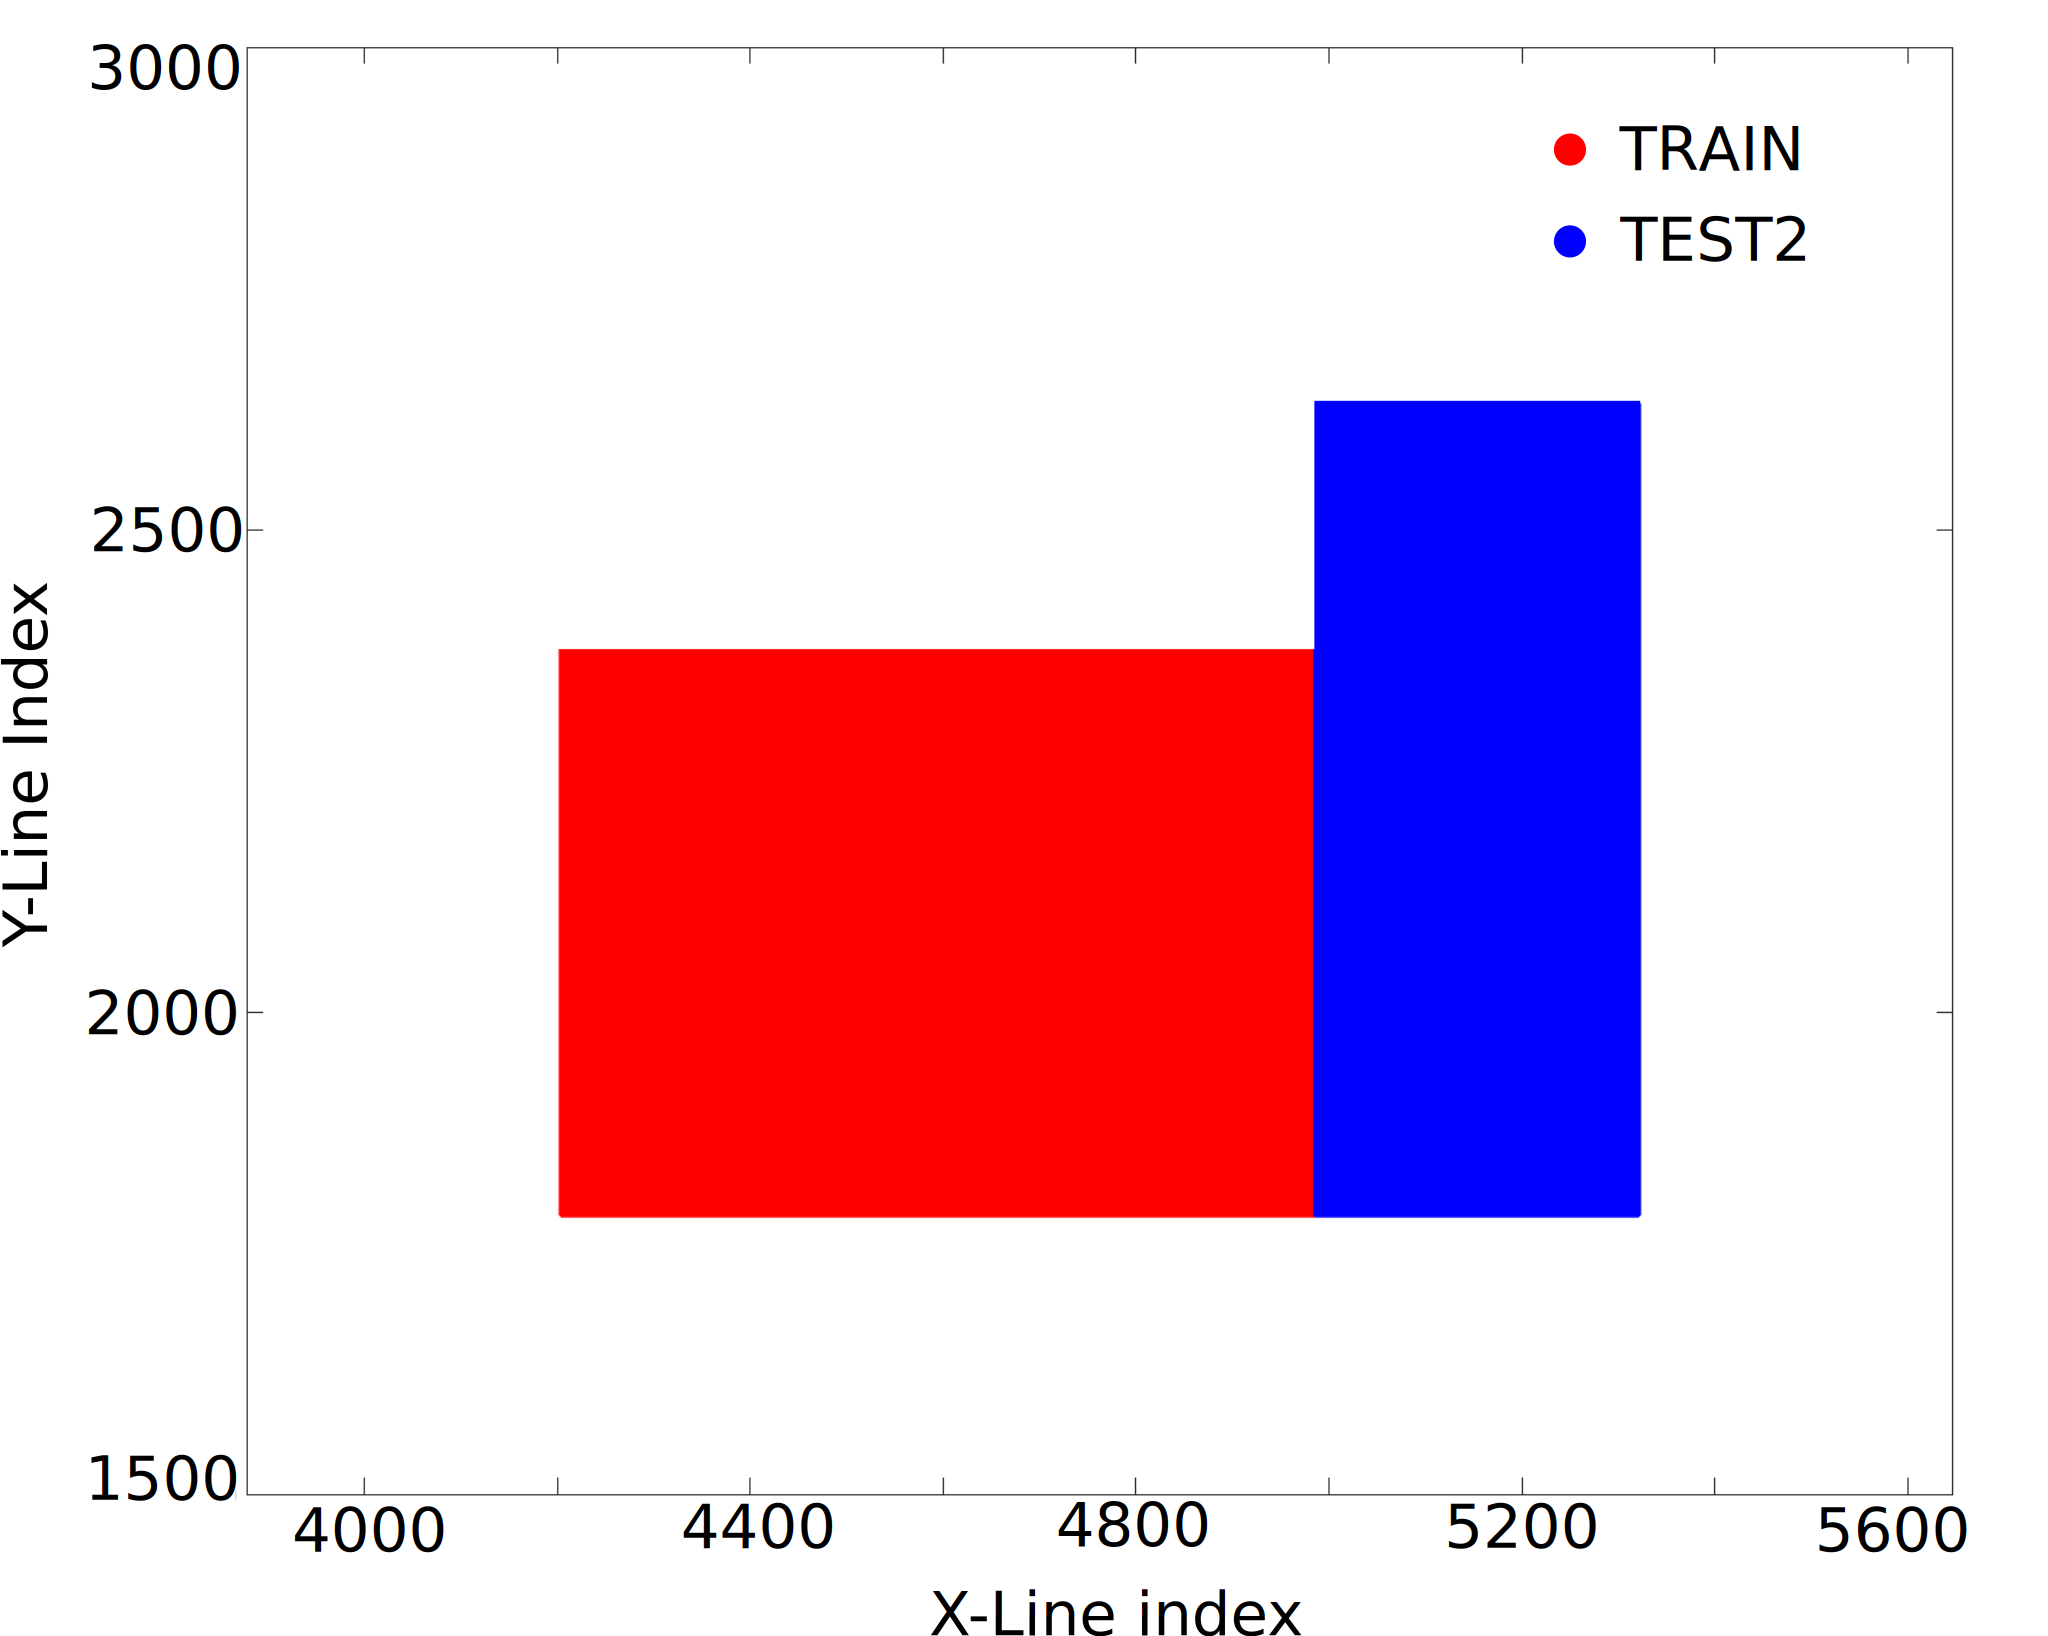
\includegraphics[width=\columnwidth]{Figures/parahika_block.pdf}
	\caption{View looking down on the XY plane showing how the training and test data sets fit together spatially. The two data sets are extractions of a much larger 3D seismic image of the survey region, which is in the Parihaka block of the Taranaki Basin of the northwest coast of New Zealand. The absolute (X, Y) indices in this plot come from the indexing used as the local coordinate system full seismic image (adpted from \citet{seismicchalenge(2020)}).}
	\label{fig:parahika_bloco}
\end{figure}

Next, we generate labeled samples along by taking
the seismic interpretation samples made of human-interpreters who identified 6 such facies to label around the red area (Figure \ref{fig:parahika_bloco}) as input and the associated facies label as output.
Figure \ref{fig:label_distribution} shows the facies class distribution.
As shown, the training set consists of 782 labeled samples. Such a number of diverse labeled samples would allow us to perform classification using supervised CNNs.
\begin{figure}[h!]
	\centering
	\includegraphics[width=\columnwidth]{Figures/label_distribution.pdf}
	\caption{Training label distribution with 782 samples divided in 6 geological classification, represented by the above 6 colors.}
	\label{fig:label_distribution}
\end{figure}

Figure \ref{fig:loss_accuracy} shows the training history using the \citet{3dFacies(2021)} coding with a batch size of 8 and a learning rate of 0.00085. 
Based on the training history, we choose the ideal point to stop training at approximately 40 epochs to minimize the possibility of lost connection, since, all programming was done through cloud processing. 
The prediction accuracy achieved the validation score 0.73, and the F1 score is 0.65.

Following the supervised training, we perform prediction on on blue Parahika block (Figure \ref{fig:parahika_bloco}) using the trained model. 
Figures \ref{fig:predict_part1} and \ref{fig:predict_part2} show several slices from predicted facies with their respective seismic slice.

\section{Conclusions}


We applied a deep neural network framework for 3D seismic facies classification calibrated from geologic interpretation. 
The CNNs are powerful and efficient for feature representation using seismic data and, thus, provide more accurate seismic facies characterization.
Validation of field data shows the potential of the method, and in future work, we plan to integrate, well log data in the workflow, interpretation of other structural features such as faults or salt bodies and other basins around the world.


\section{Acknowledgment} 

On behalf of the Geosciences Institute (UFPa), I would like to thank my colleagues in the petrophysics research group, Professor Jadsom Sampaio, Professor Carolina Barros, and CAPES, that provide me the scholarship.

\bibliography{Bibli}

\begin{figure*}[ht!]
	\centering
	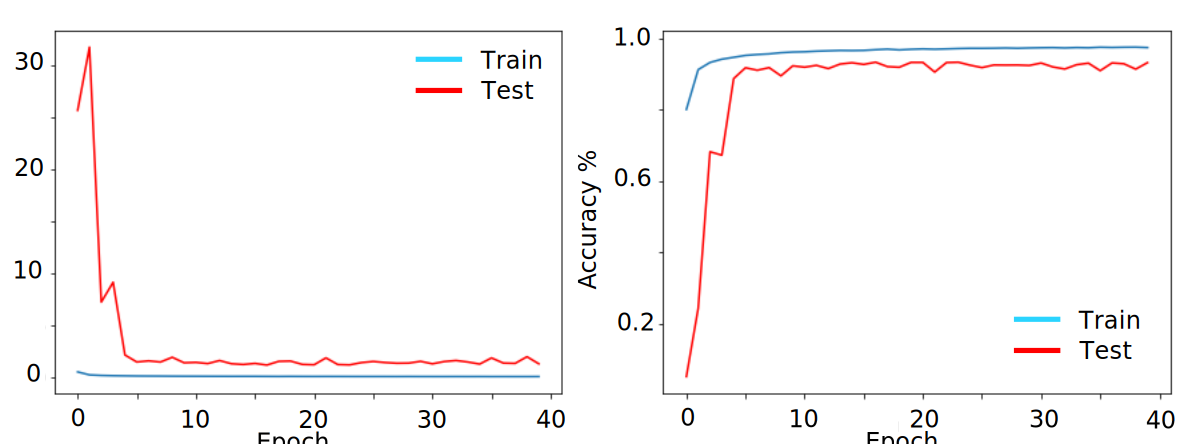
\includegraphics[width=18cm]{Figures/loss_accuracy.pdf}
	\caption{Training label distribution with 782 samples divided in 6 geological classification, represented by the above 6 colors.}
	\label{fig:loss_accuracy}
\end{figure*}

\begin{figure*}[ht!]
	\centering
	\includegraphics[width=8cm]{Figures/predict1.png}
	\includegraphics[width=8cm]{Figures/seismic1.png}
	\includegraphics[width=8cm]{Figures/predict100.png}
	\includegraphics[width=8cm]{Figures/seismic100.png}
	\includegraphics[width=8cm]{Figures/predict200.png}
	\includegraphics[width=8cm]{Figures/seismic200.png}

	\caption{Stratigraphy slices predictions (left) and its respective seismic slice sample. Samples 1, 100 and 200.}
	\label{fig:predict_part1}
\end{figure*}
\begin{figure*}[ht!]
	\centering
	\includegraphics[width=8cm]{Figures/predict300.png}
	\includegraphics[width=8cm]{Figures/seismic300.png}
	\includegraphics[width=8cm]{Figures/predict334.png}
	\includegraphics[width=8cm]{Figures/seismic334.png}
	
	\caption{Stratigraphy slices predictions (left) and its respective seismic slice sample. Samples 300 and 334.}
	\label{fig:predict_part2}
\end{figure*}


\end{document}
